\documentclass[a4paper,12pt]{article}

\usepackage{graphicx} % Required for inserting images
\usepackage{amsmath,amssymb,amsfonts}
\usepackage{subcaption}
% -----------------------
% Package Imports
% -----------------------

% Set page margins
\usepackage[a4paper, top=1in, bottom=0.8in, left=1.1in, right=0.8in]{geometry}

% Use Times New Roman font
\usepackage{times}

% Add page numbering
\pagestyle{plain}
\usepackage{multirow}
% Enable graphics inclusion
\usepackage{graphicx}
\usepackage{float}
% Enable code listings
\usepackage{listings}
\usepackage{xcolor} % For customizing code colors

% Define MATLAB style for listings
\lstdefinestyle{vscode-light}{
	language=Matlab,
	basicstyle=\ttfamily\footnotesize,
	keywordstyle=\color{blue},
	commentstyle=\color{gray},
	stringstyle=\color{red},
	numberstyle=\tiny\color{black},
	numbersep=5pt,
	frame=single,
	backgroundcolor=\color{white!10},
	breaklines=true,
	captionpos=b,
	tabsize=4,
	showstringspaces=false,
	numbers=left,  % Enable line numbering on the left
	stepnumber=1,  % Line numbers increment by 1
	numberfirstline=true, % Number the first line
}
\setlength{\parindent}{0pt}
\begin{document}
	\section{Experiment No. 1}
	
	\section{Experiment Title }
	Introduction to MATLAB and performing algebraic and matrix manipulations using MATLAB
	\section{Objective}
	
The objectives of this lab are to:
\begin{itemize}
\item To learn MATLAB basics.
\item To plot the Fourier series of a square wave.
\item To calculate the average of test marks using matrices.
\item To use user-defined functions in MATLAB.
\end{itemize}
	\section{Theory}
	




	This lab report explores MATLAB's computational capabilities through three distinct tasks: approximating a square wave via its Fourier series, performing matrix operations to calculate the average of test marks, and implementing user-defined functions to modularize code. Each section provides the theoretical background, detailed MATLAB code, and a discussion of the outcomes.


\section{Introduction to MATLAB}
\subsection{Theory and MATLAB Code}


MATLAB, short for \textbf{Matrix Laboratory}, is a powerful and versatile tool used for mathematical calculations, data analysis, and scientific computing. It is designed to handle complex mathematical operations efficiently and provides a great environment for performing calculations, visualizing data, and developing algorithms. MATLAB is widely used in engineering, science, and economics for tasks like solving equations, analyzing data, and creating models.

MATLAB's primary strength lies in its ability to work with matrices and perform operations on them easily, making it the natural choice for computational mathematics. Additionally, it provides built-in graphics tools that make it easy to plot data and visualize mathematical functions, which are key for data analysis and research. The MATLAB desktop environment encourages users to experiment and explore different ideas and solutions.

MATLAB is also flexible in integrating with other programming languages like Java, C/C++, and .NET, allowing users to combine MATLAB's power with other languages for building applications and systems.

\subsection*{Key Features of MATLAB}
MATLAB is commonly used for various tasks in different fields, including:

\begin{enumerate}
	\item \textbf{Mathematical Computations:} MATLAB supports a wide range of mathematical operations, including matrix operations, solving equations, performing integrals and derivatives, Fourier transforms, and basic statistics.
	\item \textbf{Data Visualization:} MATLAB allows the creation of 2D and 3D plots, graphs, and animations to visualize data and mathematical functions. It also supports image processing.
	\item \textbf{Programming and Automation:} MATLAB lets users write scripts and functions to automate calculations and processes. It offers features like control flow, loops, and error handling for efficient programming.
	\item \textbf{Data Import/Export:} MATLAB can import and export data from various formats such as spreadsheets, text files, and databases. It also supports big data and web data retrieval.
	\item \textbf{App Development:} Users can develop interactive applications using MATLAB’s tools like GUIDE and App Designer. Apps can be used for data analysis, modeling, and more.
	\item \textbf{Advanced Software Development:} MATLAB allows object-oriented programming, testing, debugging, and optimization. It also supports connecting to external systems like hardware or other software.
	\item \textbf{Hardware Integration:} MATLAB can be integrated with third-party hardware such as sensors, Arduino, and Raspberry Pi for real-time data processing.
\end{enumerate}


\subsection*{MATLAB Window Components}
The main window in MATLAB is divided into several panels:

\begin{enumerate}
	\item \textbf{Current Folder:} This panel shows the directory where files are located. We can navigate through our computer's file system here.
	\item \textbf{Command Window:} This is the area where we type commands and execute them. The prompt $(>>)$ indicates that MATLAB is ready to accept a command.
\end{enumerate}
\begin{figure}[H]
	\centering
	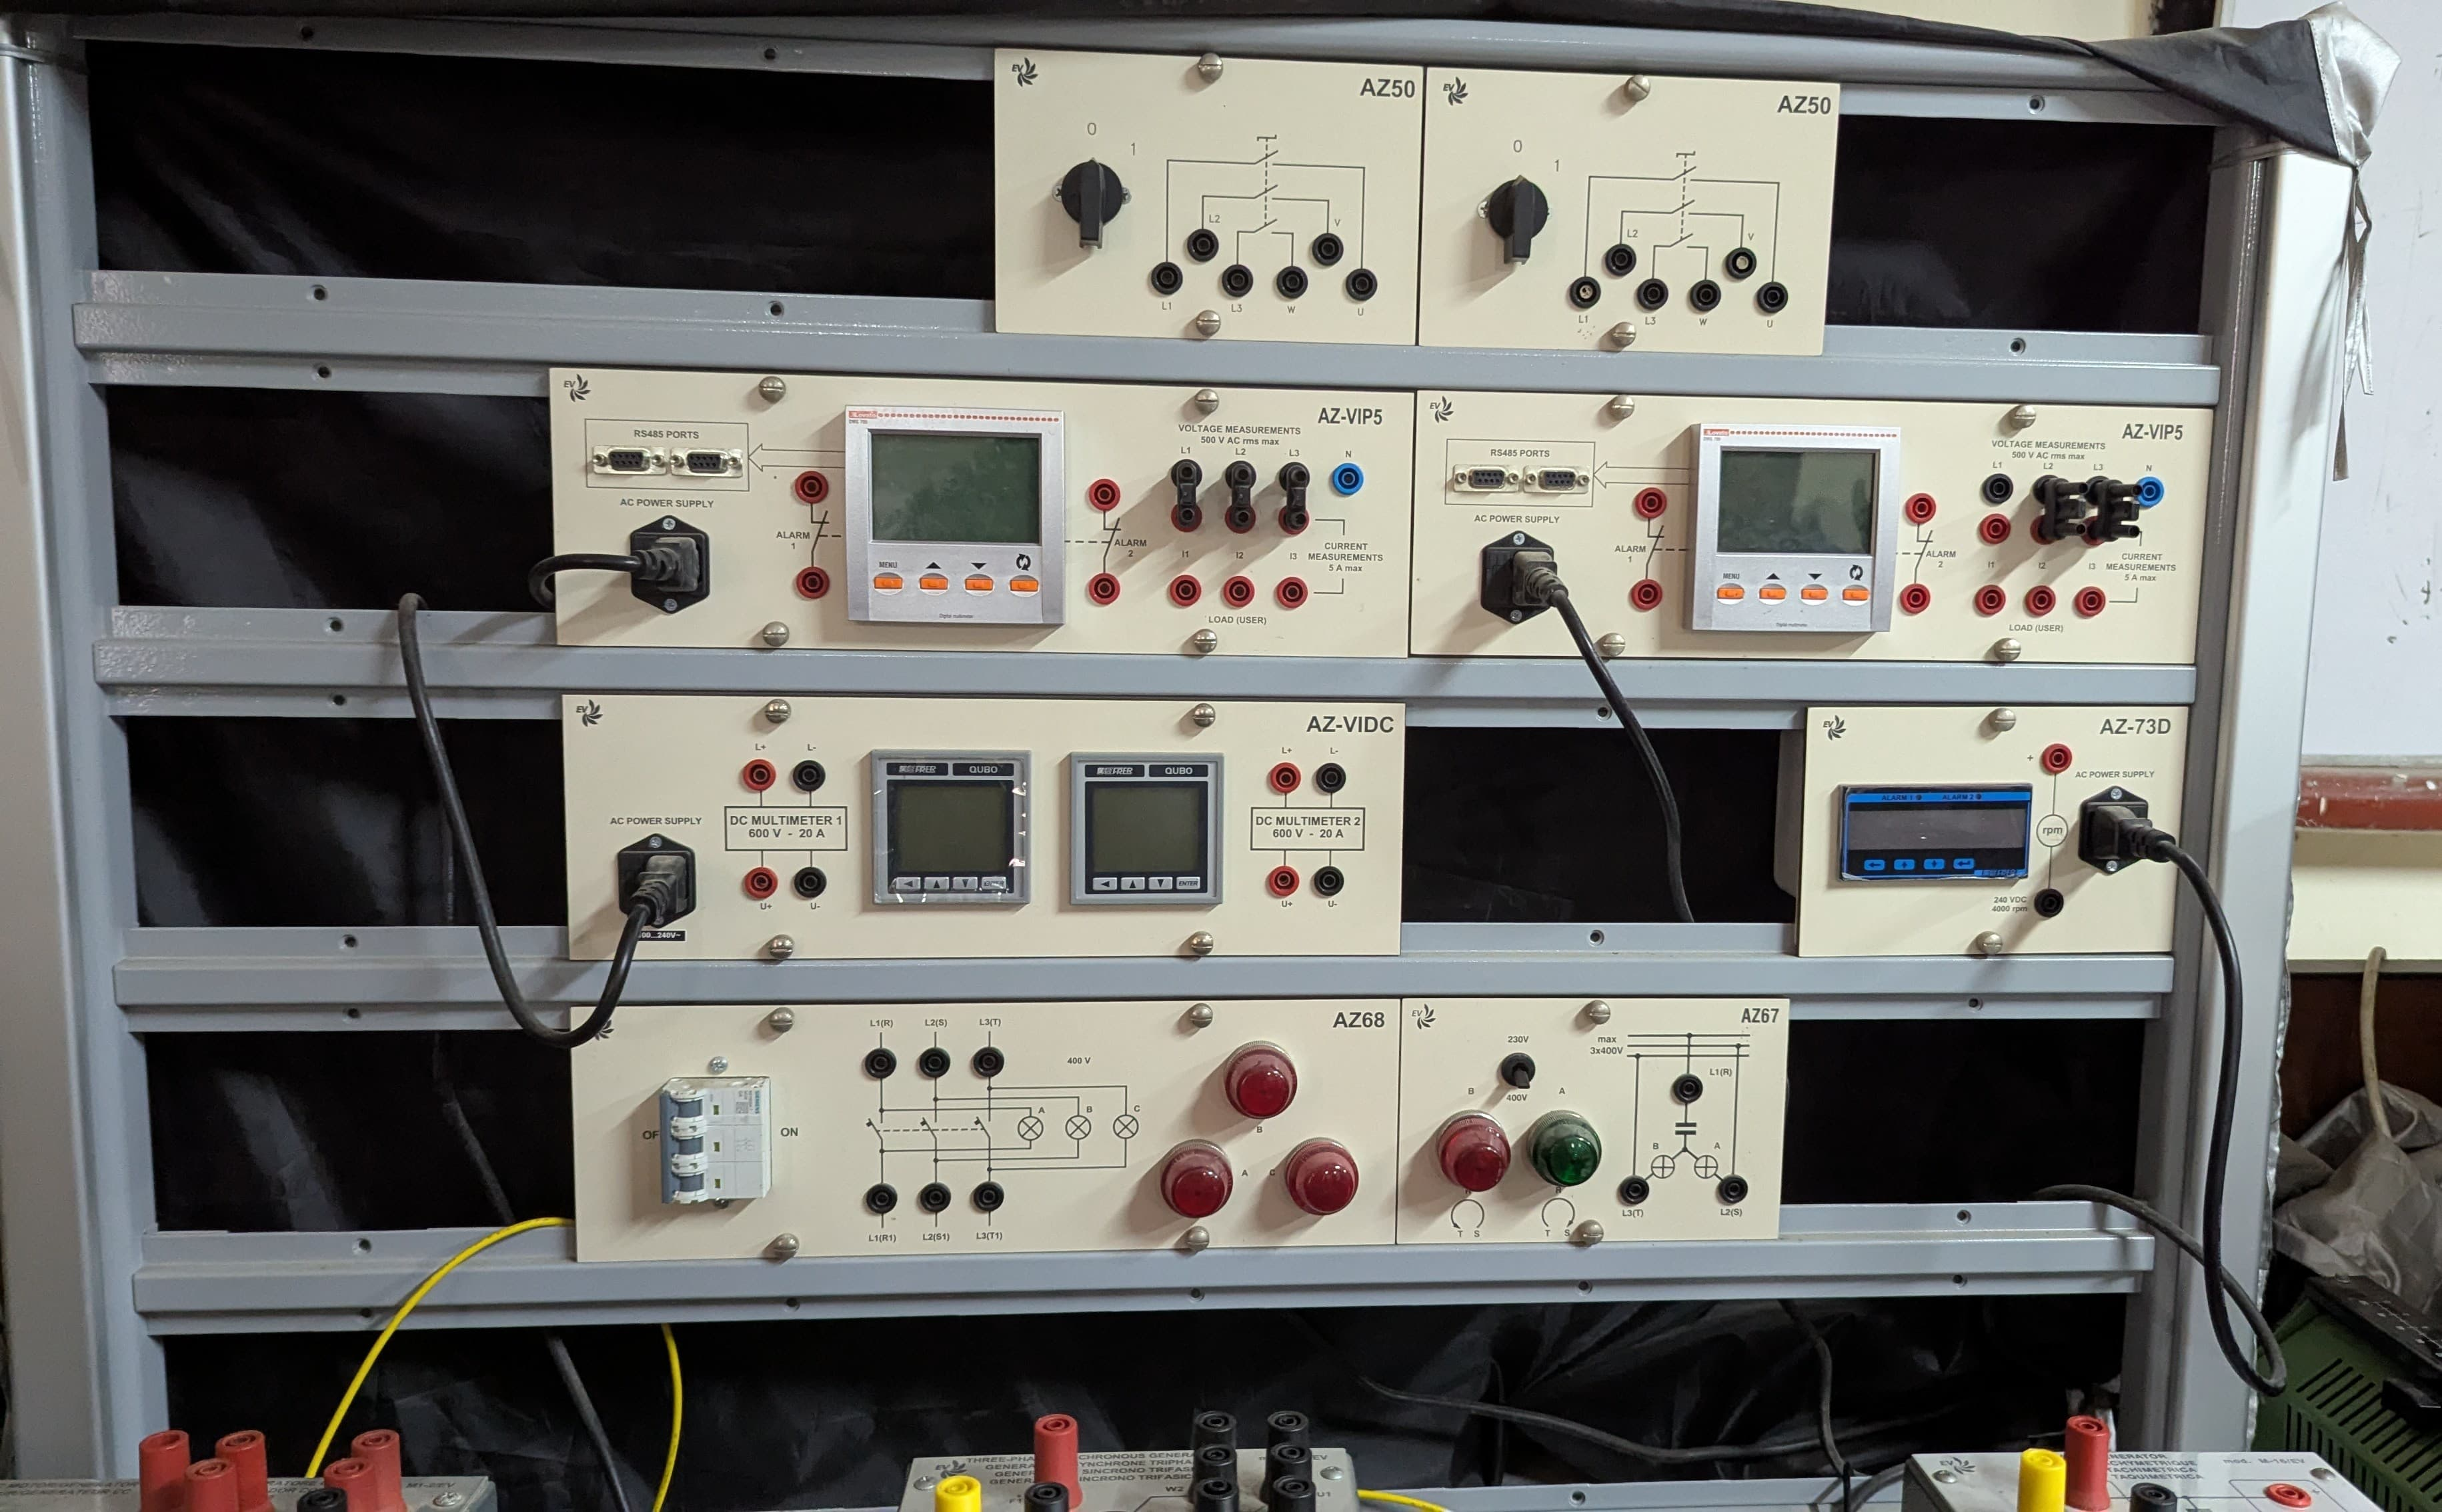
\includegraphics[width=1\linewidth, height=0.4\textheight]{Images/4}
	\caption{Opening window in MATLAB}
	\label{fig:screenshot002}
\end{figure}
\subsection*{Basic MATLAB Commands}
There are several useful commands in MATLAB that help manage our workspace, run code, and get help:

\begin{enumerate}
	\item \texttt{clc}: Clears the command window, removing previous outputs and messages.
	\item \texttt{clear}: Clears all variables from the workspace, freeing up memory.
	\item \texttt{close}: Closes any open figure or plot windows.
	\item \texttt{help}: Provides information about a specific MATLAB function. For example, typing \texttt{help sum} will give details on how to use the \texttt{sum} function.
	\item \texttt{doc}: Opens the full MATLAB documentation for a specific function. It gives detailed descriptions and examples.
	\item \texttt{pwd}: Displays the current working directory where MATLAB is looking for files.
	\item \texttt{cd}: Changes the current directory. For example, \texttt{cd('C:/Documents')} will change the directory to the specified folder.
	\item \texttt{save}: Saves the current variables in the workspace to a file for later use.
	\item \texttt{load}: Loads variables from a saved file into the workspace.
\end{enumerate}

\subsection*{Workspace}
The \textbf{Workspace} is where all the variables we create and manipulate are stored. It acts as the memory for MATLAB, allowing us to keep track of our data, intermediate results, and final outputs. We can see a list of all variables in the workspace and manage them from the workspace panel.

MATLAB's environment is designed to be user-friendly, and it encourages users to experiment with different commands, functions, and scripts. Whether  solving math problems, visualizing data, or designing systems, MATLAB makes these tasks easier with its rich set of tools and features.


\subsection{Basic Matrix Manipulations}

In this section, we will cover various matrix manipulations in MATLAB, including creating matrices, performing arithmetic operations, and working with matrix dimensions.

\subsection*{Matrix of Zeros}
A matrix of zeros can be created using the \texttt{zeros} function. For example, to create a 3x3 matrix of zeros:
\begin{lstlisting}[style=vscode-light]
	A = zeros(3, 3);
\end{lstlisting}
The resulting matrix \( A \) will be:
\[
A = \begin{bmatrix}
	0 & 0 & 0 \\
	0 & 0 & 0 \\
	0 & 0 & 0
\end{bmatrix}
\]

\subsection*{Matrix of Ones}
A matrix of ones can be created using the \texttt{ones} function. For example, to create a 3x2 matrix of ones:
\begin{lstlisting}[style=vscode-light]
	B = ones(3, 2);
\end{lstlisting}
The resulting matrix \( B \) will be:
\[
B = \begin{bmatrix}
	1 & 1 \\
	1 & 1 \\
	1 & 1
\end{bmatrix}
\]

\subsection*{Identity Matrix}
An identity matrix can be created using the \texttt{eye} function. For example, to create a 4x4 identity matrix:
\begin{lstlisting}[style=vscode-light]
	C = eye(4);
\end{lstlisting}
The resulting matrix \( C \) will be:
\[
C = \begin{bmatrix}
	1 & 0 & 0 & 0 \\
	0 & 1 & 0 & 0 \\
	0 & 0 & 1 & 0 \\
	0 & 0 & 0 & 1
\end{bmatrix}
\]

\subsection*{Matrix of Random Numbers}
A matrix of random numbers can be created using the \texttt{rand} function. For example, to create a 4x2 matrix of random numbers:
\begin{lstlisting}[style=vscode-light]
	D = rand(4, 2);
\end{lstlisting}
The resulting matrix \( D \) might look like:
\[
D = \begin{bmatrix}
	0.4981 & 0.7386 \\
	0.9009 & 0.5860 \\
	0.5747 & 0.2467 \\
	0.8452 & 0.6664
\end{bmatrix}
\]

\subsection*{Size of a Matrix}
To find the size of a matrix, we use the \texttt{size} function. For example:
\begin{lstlisting}[style=vscode-light]
	size_B = size(B);
\end{lstlisting}
The result will be:
\[
\text{size\_B} = [3, 2]
\]
This indicates that matrix \( B \) has 3 rows and 2 columns.

\subsection*{Transpose of a Matrix}
The transpose of a matrix can be found using the \texttt{'} operator. For example:
\begin{lstlisting}[style=vscode-light]
	Trans = D';
\end{lstlisting}
The resulting matrix \( Trans \) will be:
\[
Trans = \begin{bmatrix}
	0.4981 & 0.9009 & 0.5747 & 0.8452 \\
	0.7386 & 0.5860 & 0.2467 & 0.6664
\end{bmatrix}
\]

\subsection*{Creating a Matrix}
Matrices can be created directly by specifying the elements. For example:
\begin{lstlisting}[style=vscode-light]
	b = [2 -4 5; 1 2 5; 5 0 1];
\end{lstlisting}
The resulting matrix \( b \) will be:
\[
b = \begin{bmatrix}
	2 & -4 & 5 \\
	1 & 2 & 5 \\
	5 & 0 & 1
\end{bmatrix}
\]

\subsection*{Matrix Addition}
Matrices of the same size can be added element-wise. For example, if \( a \) and \( b \) are two matrices of the same size:
\begin{lstlisting}[style=vscode-light]
	sum = a + b;
\end{lstlisting}
The resulting matrix \( sum \) will be:
\[
sum = \begin{bmatrix}
	2.0835 & -3.2702 & 5.7690 \\
	1.6260 & 2.8908 & 5.5814 \\
	5.6609 & 0.9823 & 1.9283
\end{bmatrix}
\]

\subsection*{Matrix Subtraction}
Matrices of the same size can be subtracted element-wise. For example:
\begin{lstlisting}[style=vscode-light]
	sub = a - b;
\end{lstlisting}
The resulting matrix \( sub \) will be:
\[
sub = \begin{bmatrix}
	-1.9165 & 4.7298 & -4.2310 \\
	-0.3740 & -1.1092 & -4.4186 \\
	-4.3391 & 0.9823 & -0.0717
\end{bmatrix}
\]

\subsection*{Matrix Multiplication}
Matrix multiplication is performed using the \texttt{*} operator. For example:
\begin{lstlisting}[style=vscode-light]
	multi = a * b;
\end{lstlisting}
The resulting matrix \( multi \) will be:
\[
multi = \begin{bmatrix}
	4.7419 & 1.1256 & 4.8352 \\
	5.0499 & -0.7223 & 8.1650 \\
	6.9458 & -0.6792 & 9.1446
\end{bmatrix}
\]

\subsection*{Element-wise Multiplication}
Element-wise multiplication of matrices can be done using the \texttt{.*} operator. For example:
\begin{lstlisting}[style=vscode-light]
	emulti = a .* b;
\end{lstlisting}
The resulting matrix \( emulti \) will be:
\[
emulti = \begin{bmatrix}
	0.1670 & -2.9190 & 3.8451 \\
	0.6260 & 1.7815 & 2.9072
\end{bmatrix}
\]
\newpage
\subsection{Calculating and Plotting the Fourier Series of a Square Wave}

\subsubsection*{Theory}
A Fourier series expresses a periodic function as a sum of sines and cosines. For a square wave, only sine terms with odd harmonics contribute. The Fourier series approximation is given by:
\[
f(t) = \frac{4}{\pi} \sum_{n=1,3,5,\dots}^{N} \frac{1}{n} \sin(2\pi fnt)
\]
where \( N \) represents the number of terms. Increasing \( N \) enhances the accuracy of the approximation, although discontinuities exhibit the Gibbs phenomenon.

\subsubsection*{MATLAB Code}
\begin{lstlisting}[style=vscode-light, caption={Fourier Series Approximation of a Square Wave} ]

	% Fourier Series Approximation of a Square Wave
clc % Clears command window
clear % Clears workspace

%%%%%%%%%%%%%%%%%%%%%%%%%%%%%%%%%%%%%%%%%%%%%%
f = 1; % Declare frequency of square wave
t = 0:0.001:2; % Take the timespan and time step
y = 1*square(2*pi*f*t); % Function for square wave
plot(t,y,'LineWidth',2) % Plot square wave
hold on % Hold on to plot another %waveshape in same figure
%% Calculating and plotting Fourier series up to 50th order
N = 50;
y50 = 0;

for n = 1:2:N
y50 = y50+(4/pi)*(1/n)*sin(2*pi*f*t*n);
end
plot(t,y50,'LineWidth',2);

%% Calculating and plotting Fourier series up to 5th order
N = 7;
y7 = 0;
for n = 1:2:N
y7 = y7+(4/pi)*(1/n)*sin(2*pi*f*t*n);
end
plot(t,y7,'LineWidth',2)

%% Calculating and plotting Fourier series up to 2nd order
N = 3;
y3 = 0;
for n = 1:2:N
y3 = y3+(4/pi)*(1/n)*sin(2*pi*f*t*n);
end
plot(t,y3,'LineWidth',2)

%% Setting up legend, x-label and y-label
legend('Square wave','Order= 50','Order= 7','Order= 3')
xlabel('Time (t) (Seconds)')
ylabel('Amplitude')
title('Fourier Analysis of a Square Wave')

\end{lstlisting}

\subsection{Figure}

\begin{figure}[H]
	\centering
	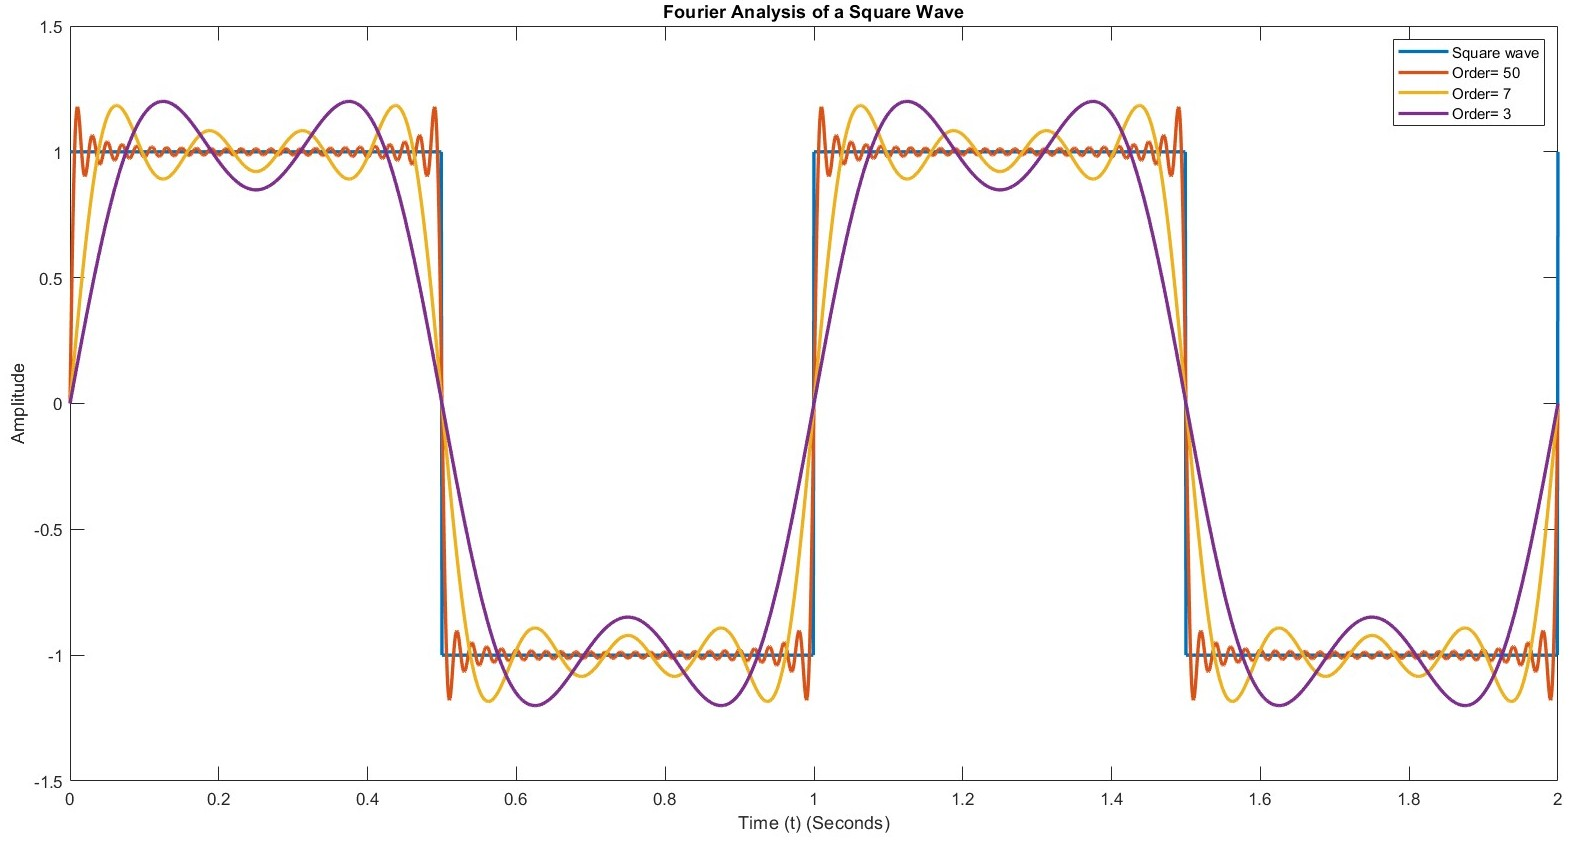
\includegraphics[width=1\linewidth]{Images/fourier_series4}
	\caption{Plot of the original square wave with its Fourier series of order 50, 7, and 3}
	\label{fig:screenshot002}
\end{figure}

\subsection{Matrix Manipulation: Calculating Average Test Marks}

\subsubsection*{Theory}
MATLAB excels at matrix operations, enabling efficient data processing. In this task, we store test marks in a matrix where each row corresponds to a student and each column to a test. The \texttt{mean} function is used to compute both the average per student (row-wise) and the overall average mark.

\begin{table}[H]
		\centering
	\caption{Calculating Average Test Marks }
	\begin{tabular}{|c|c|c|c|c|}
		\hline
		Roll Number & CT1 & CT2 & CT3 & CT4 \\ \hline
		2101071     & 11  & 20  & 20  & 20  \\ \hline
		2101072     & 12  & 14  & 14  & 19  \\ \hline
		2101073     & 13  & 16  & 10  & 18  \\ \hline
		2101074     & 14  & 17  & 12  & 17  \\ \hline
		2101076     & 15  & 19  & 11  & 16  \\ \hline
		2101077     & 16  & 19  & 4   & 15  \\ \hline
		2101078     & 17  & 19  & 10  & 14  \\ \hline
		2101081     & 18  & 18  & 17  & 16  \\ \hline
	\end{tabular}
\end{table}
\newpage
\subsubsection{MATLAB Code}
\begin{lstlisting}[style=vscode-light, caption={Calculating Average Test Marks Using Matrices} ]
clc %Clears command window.
clear %Clears workspace.

%Change directory. Location of %excel file in cd()function.
cd('D:\DOWNLOAD 2024 V2\LATEX FILE\3.1');
%Writes the excel file named "ctmark" into matrix "a".
a=xlsread('ctmark'); 
%Writes 1st column of a matrix ,roll numbers into b matrix.
b=a(:,1)
%Writes 2nd to 5th columns of a matrix i.e.,CT marks %into c matrix.
c=a(:,2:5)
%t is the transpose matrix of c matrix. So, the comlumns %become rows.
t=c'; 
%"sort" function sotrs each column in descending order.
d=sort(t,'Descend') 
%Transpose matrix of d matrix becomes e matrix. So, the %columns becomes rows.
e=d' 
%Writes 1st to 3rd columns of e matrix
f=e(:,1:3) 
%"sum" function adds all of it's columns and writes %them in s matrix. 
s=sum(f,2)
%Dividing each entry of s matrix and writing the result %into avg matrix. avg matrix is the average CT mark of each %student.
avg=s/3 
%Rounds the average value upto 3 digits %after decimal sign.
result =round(avg,3)
%Entries of b matrix, the matrix containing %roll numbers of each student is converted into string by
Roll=num2str(b) 

% Prepare the data to be displayed as a table
CT1 = c(:,1); % First CT marks.
CT2 = c(:,2); % Second CT marks.
CT3 = c(:,3); % Third CT marks.
CT4 = c(:,4); % Fourth CT marks.

% Create the table with the data
T = table(Roll, CT1, CT2, CT3, CT4, result, 'VariableNames', {'Roll Number', 'CT1', 'CT2', 'CT3', 'CT4', 'Average Number'});
% Display the table in the command window
disp(T);



\end{lstlisting}
\subsection{Result Shown in Command Window}
\begin{table}[H]
	\centering
	\begin{tabular}{llllll}
		Roll Number            & CT1    & CT2    & CT3    & CT4    & Average Number               \\
		\_\_\_\_\_\_\_\_\_\_\_ & \_\_\_ & \_\_\_ & \_\_\_ & \_\_\_ & \_\_\_\_\_\_\_\_\_\_\_\_\_\_ \\
		2101071                & 11     & 20     & 20     & 20     & 20                           \\
		2101072                & 12     & 14     & 14     & 19     & 15.667                       \\
		2101073                & 13     & 16     & 10     & 18     & 15.667                       \\
		2101074                & 14     & 17     & 12     & 17     & 16                           \\
		2101076                & 15     & 19     & 11     & 16     & 16.667                       \\
		2101077                & 16     & 19     & 4      & 15     & 16.667                       \\
		2101078                & 17     & 19     & 10     & 14     & 16.667                       \\
		2101081                & 18     & 18     & 17     & 16     & 17.667                       \\
		&        &        &        &        &                             
	\end{tabular}
\end{table}
\subsection{User-Defined Functions in MATLAB}

\subsubsection*{Theory}
User-defined functions in MATLAB allow us to create reusable pieces of code. In this example, we define a function \texttt{celsiusToFahrenheit} that converts a temperature from Celsius to Fahrenheit, using user input. This modular approach allows the conversion logic to be reused easily in other parts of the program.

\subsubsection{MATLAB Code: Function File}
Save the following code in a file named \texttt{celsiusToFahrenheit.m}.
\begin{lstlisting}[style=vscode-light, caption={User-Defined Function: celsiusToFahrenheit.m}]
	function fahrenheit = celsiusToFahrenheit(celsius)
	% celsiusToFahrenheit converts a temperature from Celsius to Fahrenheit.
	% Input:
	%   celsius - temperature in Celsius
	% Output:
	%   fahrenheit - temperature in Fahrenheit
	
	fahrenheit = (celsius * 9/5) + 32;
	end
\end{lstlisting}

\subsubsection*{MATLAB Code: Main Script Using the Function with User Input}
\begin{lstlisting}[style=vscode-light, caption={Using the User-Defined Function with User Input}]
	% Using the user-defined function to convert Celsius to Fahrenheit based on user input
	clear; clc;
	% Ask the user to input a temperature in Celsius
	celsius = input('Enter temperature in Celsius: ');
	% Call the function to convert to Fahrenheit
	fahrenheit = celsiusToFahrenheit(celsius);
	% Display the result
    disp(fahrenheit);
\end{lstlisting}




\section{Discussion}
In this sessional, an introduction to MATLAB was provided, focusing on its capabilities for algebraic operations and plotting. MATLAB was used to calculate and visualize the Fourier series of a square wave, demonstrating its power for mathematical computations and graphical representation. Basic matrix manipulations were also covered, such as creating matrices and calculating averages, which were applied to compute the average of class test marks. Additionally, user-defined functions were created for temperature conversion, emphasizing the flexibility of MATLAB for custom functions. Overall, the session successfully met its objectives and provided foundational skills for working with MATLAB.



	
	
	
\end{document}